\chapter{EXPERIMENTS}

% Ubah bagian-bagian berikut dengan isi dari pengujian dan analisis

%Pada bab ini, akan dipaparkan pengaruh modifikasi-modifikasi yang dilakukan pada YOLOv7.
\section{Baseline Performance}
For comparison purposes, we first measure the baseline performance of YOLOv7 with all
modification candidates from section \ref{section:modificationcandidates} stripped.
We call this model as \verb|YOLOv7-plain|.
After 300 epochs of training with batch-size 1 like in the experiment setup, we found that
this model was unable to detect anything on the test set (a valid detection is detection with $IoU>0.5$ to groundtruth). 
%Untuk mengukur pengaruh dari modifikasi-modifikasi yang dilakukan pada YOLOv7, maka
%hal pertama yang harus dilakukan adalah mengukur performa YOLOv7 tanpa segala modifikasi
%yang diajukan pada bab \ref{section:modificationcandidates}. Arsitektur YOLOv7 \emph{plain} 
%ini di-\emph{train} pada 400 sampel data dari  \textcite{aot_dataset} dengan 300 epoch dan batch size 1.
%Dengan aturan tersebut, ditemukan bahwa model \emph{plain} tidak mampu untuk mendeteksi
%objek apapun pada dataset uji, dengan kriteria "terdeteksi" $IoU > 0.5$ (mAP@.5 = 0).
%
%Untuk keperluan komparasi dengan performa-performa dari modifikasi pada YOLOv7,
%model \emph{plain} ini akan selanjutnya disebut sebagai \verb*|YOLOv7-plain|.

\section{Mosaic Augmentation and Anchor Recalculation}


%Terdapat 3 modifikasi yang diujikan pada bagian ini, yaitu \verb*|YOLOv7-plain| yang ditambahkan augmentasi mosaic,
%\verb*|YOLOv7-plain| yang direkalkulasi anchor, dan \verb*|YOLOv7-plain| yang ditambahkan augmentasi mosaic dan rekalkulasi anchor.
In this section, we present the effect of mosaic augmentation and anchor recalulation on the $mAP@50$ score when applied
independently and combinatively. For comparison purposes, we assigned names the models as \verb|YOLOv7-M|,
\verb|YOLOv7-AR|, and \verb|YOLOv7-MAR|. These names correspond to \verb|YOLOv7-plain| with mosaic augmentation, \verb|YOLOv7-plain|
with anchor recalculation, and \verb|YOLOv7-plain| with both mosaic augmentation and anchor recalculation, respectively.
%\subsection{Augmentasi Mosaic}

The process of applying mosaic augmentation to the dataset is pretty straightforward as YOLOv7's implementation code
already provide the mosaic augmentation tool. A mosaic augmentation result example can be seen in Figure \ref{fig:mosaic-train}.
  %Proses melakukan augmentasi mosaic cukup \emph{straightforward},
  %augmentasi ini dilakukan pada beberapa data training.
  %Contoh hasil augmentasi dapat dilihat pada gambar \ref{fig:mosaic-train}
  \begin{figure}
    \centering
    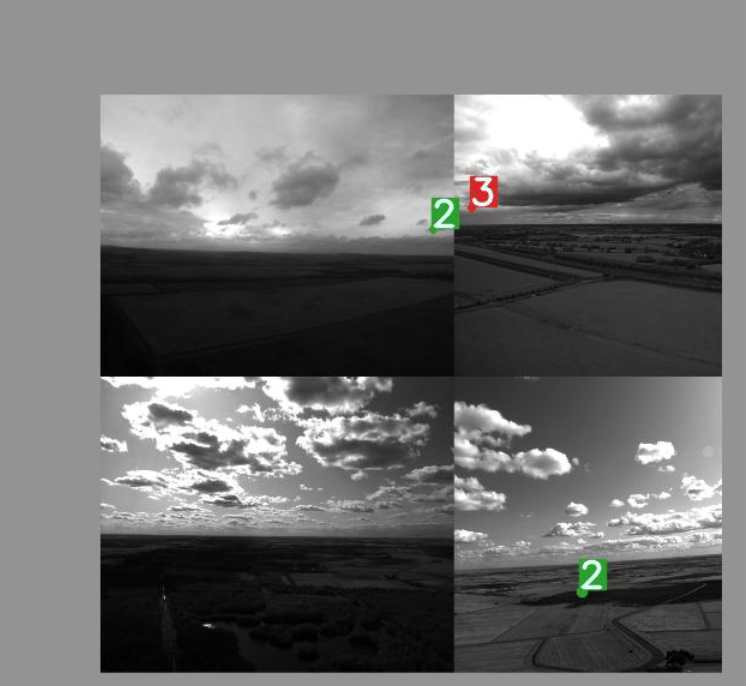
\includegraphics[scale=0.4]{figures/mosaic-aug-2.png}
    \caption{An example of mosaic augmented image}
    \label{fig:mosaic-train}
  \end{figure}

  %, sedangkan untuk rekalkulasi anchor akan dibahas pada bagian berikut.
%\subsection{Rekalkulasi Anchor}
%Rekalkulasi anchor dilakukan dengan mengklaster data training ke 9 centroid menggunakan algoritma k-means.
Anchor recalculation is done by clustering the training data's widths and heights to 9 centroid using k-means algorithm.
However, due to the skewed distribution of the dataset, regular k-means (with $L^2$ Distance) actually failed to form 9 clusters.
To fix this, we used a distance function
\begin{equation} 
  L = \sqrt{\ln^2{\frac{w_1}{w_2}} + \ln^2{\frac{h_1}{h_2}}}
  \label{eq:logdistancefunc}
\end{equation}
Distance function in equation \ref{eq:logdistancefunc} was actually an $L^2$ distance but with log-transformed space.
With this function, k-means was finally able to cluster the data into 9 centroids.
These centroids are used by the head layers as anchors. Each head uses 3.
The comparison of the original anchor and recalculated anchor can be seen in Table \ref{tbl:recalculated_anchor}
and Figure \ref{fig:anchor-dist}.
%Sembilan centroid tersebut digunakan sebagai anchor, 3 untuk tiap head pada arsitektur YOLO (terdapat 3 head).
%Persebaran anchor sebelum dan sesudah direkalkulasi dapat dilihat 
%pada Tabel \ref{tbl:recalculated_anchor} dan Gambar \ref{fig:anchor-dist}

\begin{table}
  \centering
  \captionof{table}{Anchor Points Before and After Recalculation}
  \label{tbl:recalculated_anchor}
  \vspace{-1ex}
  \begin{table}[H]
  \centering
  \captionof{table}{Titik Hasil Rekalkulasi Anchor}
  \label{tbl:recalculated_anchor}
  \vspace{-1ex}
  \begin{tabular}{ c l l }
    \toprule[1.5pt]
    Layer Head & Anchor Lama        & Hasil Rekalkulasi Anchor\\
    \midrule
    1          & [12,16], [19,36], [40,28]& [4,4], [14,5], [11,11]\\
    2          & [36,75], [76,55], [72,146]& [27,8], [18,17], [41,14]\\
    3          & [142,110], [192,243], [459,401]& [43,32], [86,27], [149,70]\\
    \bottomrule[1.5pt]
  \end{tabular}
\end{table}
\end{table}
\vspace{1ex}

\begin{figure}
  \centering
  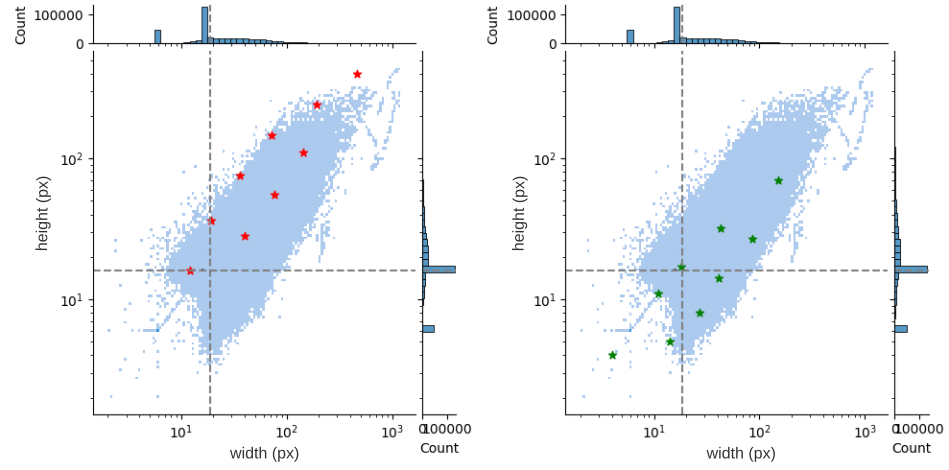
\includegraphics[width=\textwidth]{figures/anchor-dist-2.png}
  \caption{Anchor Distribution on Dataset. Left: Original Anchor. Right: Recalulated Anchors}
  \label{fig:anchor-dist}
\end{figure}

If we observe the distribution of anchors before and after recalculation in Figure \ref{fig:anchor-dist},
we can see that indeed the recalculated anchors cover more of the dataset than the original.
8 out of 9 of the original anchors are placed in the first quadrant of the median axis.
It means that those 8 anchors are responsible for only 25\% of the dataset and leave the rest to 1 anchor.
This is very inefficient. In contrast, the recalculated anchors have a more balanced distribution with
anchors distributed across each quadrant.


%Jika kita memperhatikan persebaran anchor sebelum dan sesudah direkalkulasi pada Gambar \ref{fig:anchor-dist},
%dapat kita lihat bahwa anchor hasil rekalkulasi lebih mencakup seluruh persebaran dataset daripada anchor lama.
%8 dari 9 anchor lama bertempat di kuadran pertama dari garis median(garis putus-putus).
%Hal ini berarti 8 anchor tersebut hanya mampu mendeteksi sekitar 25\% dari objek-objek pada dataset.
%Sedangkan, anchor hasil rekalkulasi menempatkan anchor di setiap kuadran.



\subsubsection{Performance}
%The performance of the 3 models compared to \verb|YOLOv7-plain| can be seen in Table \ref{tbl:mosaic_reanchor_performance}.
%We can see from the table that \verb|YOLOv7-plain| was only able to detect anything on the test set after applying both
%mosaic augmentation and anchor recalculation. With those 2 modification, the model was able to achieve 11.2\% score at mAP@50.
The performance of the three models, namely \verb|YOLOv7-M|, \verb|YOLOv7-AR|, and \verb|YOLOv7-MAR|, was compared to that of the baseline model YOLOv7-plain.
The results are presented in Table \ref{tbl:mosaic_reanchor_performance}.
It can be observed from the table that YOLOv7-plain alone was unable to detect any objects in the test set.
However, after applying both mosaic augmentation and anchor recalculation, the model achieved a notable improvement with a score of 11.2\% at mAP@50. 

\begin{table}
  \centering
  \captionof{table}{Mosaic Augmentation and Anchor Recalculation Performance}
  \label{tbl:mosaic_reanchor_performance}
  \vspace{-1ex}
    \begin{tabular}{ l l >{\hspace{4em}}c }
    \toprule[1.5pt]
    No & Model        &mAP@50 \\
    \midrule
    0  & \texttt{YOLOv7-plain}        & 0\%\\
    1  & \texttt{YOLOv7-M}            & 0\%\\
    2  & \texttt{YOLOv7-AR}           & 0\%\\
    3  & \texttt{\textbf{YOLOv7-MAR}} & \textbf{11.2}\%\\
    \midrule
       & Improvement                  & \textbf{\textcolor{green}{+11.2\%}}\\
    \bottomrule[1.5pt]
  \end{tabular}
\end{table}

Since the model \verb|YOLOv7-MAR| was the only model that was capable of detection in the test set,
we henceforth establish this model as the baseline for further modification. Meaning, in the subsequent
sections, any modifications mentioned should be presumed to be composed of mosaic augmentation and anchor recalculation,
in addition to the respective modification that was applied, unless explicitly stated otherwise.

  %Performa dari tiap modifikasi dapat dilihat pada tabel \ref{tbl:mosaic_reanchor_performance}.
  %Pada tabel tersebut, terlihat bahwa YOLOv7 mampu untuk mendeteksi beberapa objek pada dataset uji ketika diberi 
  %augmentasi mosaic pada data train dan direkalkulasi anchornya.
  %\begin{table}[H]
  \centering
  \captionof{table}{Performa Modifikasi Augmentasi Mosaic dan Rekalkulasi Anchor}
  \label{tbl:mosaic_reanchor_performance}
  \vspace{-1ex}
  \begin{tabular}{ l l c }
    \toprule[1.5pt]
    No & Modifikasi        &mAP@50 \\
    \midrule
    0  & \textbf{yolov7-plain               }& 0\%\\
    1  & \textbf{mosaic                     }& 0\%\\
    2  & \textbf{rekalkulasi anchor         }& 0\%\\
    3  & \textbf{mosaic + rekalkulasi anchor}& \textbf{11,2}\%\\
    \midrule
       & Peningkatan                         & \textbf{\textcolor{green}{+11,2\%}}\\
    \bottomrule[1.5pt]
  \end{tabular}
\end{table}

  %Hanya modifikasi nomor 3 yang mampu melakukan deteksi, maka 
  %modifikasi tersebut dijadikan baseline untuk modifikasi-modifikasi lainnya.
  %Untuk mempermudah komparasi penambahan modifikasi-modifikasi selanjutnya,
  %maka model ini akan disebut sebagai \verb*|YOLOv7-base|.

\section{Replacing Localization Loss to EIoU}
%Dengan menggunakan \verb*|YOLOv7-base| sebagai baseline, 
%Box Loss function dari YOLOv7 diganti menjadi EIoU.
%Telah juga dilakukan percobaan menggunakan convexciation pada EIoU.
%Hasil dari pengujian dapat dilihat pada Tabel \ref{tbl:loss_function_perf}
In this section, we experimented with $EIoU$.
We replaced the original $CIoU$ loss of YOLOv7 to pure $EIoU$ and convexcified version of $EIoU$.
The convexciation was done by modifying the $EIoU$ loss from $-EIoU$ to $(1-EIoU)^2$ for better
gradient dynamics during training.

The performance of these modifications can be seen in Table \ref{tbl:loss_function_perf}

\begin{table}[b]
  \centering
  \captionof{table}{EIoU Localization Loss Performance}
  \label{tbl:loss_function_perf}
  \vspace{-1ex}
    \begin{tabular}{ l l c }
    \toprule[1.5pt]
    No & Modification        &mAP@50 \\
    \midrule
    0  & \texttt{\textbf{YOLOv7-MAR +CIoU}} (original)     & \textbf{11.2}\%\\
    1  & \texttt{YOLOv7-MAR + EIoU}                & 0\%\\
    2  & \texttt{YOLOv7-MAR + EIoU + Convexication} & 4.92\%\\
    \midrule
       & Peningkatan                                & \textbf{\textcolor{red}{-6.28\%}}\\
    \bottomrule[1.5pt]
  \end{tabular}
\end{table}

Surprisingly, although $EIoU$ outperformed $CIoU$ when applied to networks like Faster-RCNN+ResNet and RetinaNet
as \textcite{eiou} claimed, it performed worse when applied to YOLOv7 with \textcite{aot_dataset}.
Even after convexciation, $CIoU$ still outperform $EIoU$ by 6.28\%.
%Ternyata, meskipun EIoU memiliki performa lebih baik daripada CIoU ketika diaplikasikan
%pada Faster-RCNN+ResNet50 dengan dataset VOC2007 dan COCO2017, EIoU tidak mampu untuk meningkatkan
%AP deteksi YOLOv7 pada dataset \textcite{aot_dataset}.

\section{Utilizing Earlier Feature Map Stage}
For this modification, we reconfigured the source of the feature map by redirecting it from P3 to P2, as shown in Figure \ref{fig:deeperconn}.
Specifically, we adjusted the routing on layer 66, changing it from 24 to 11. 
Since the output of layer 11 is at a different scale compared to 24 (with a scaling factor of $2^{-2}$ and $2^{-3}$ respectively), 
we modified the upsampling factor of layer 55 from 2 to 4 to ensure size compatibility with layer 11. 
However, this change in upsampling disrupted the subsequent layers. 
To solve this, we performed downsampling after layer 75 (connected to the head) by setting layer 77's stride to 2 and layer 79's stride to 4, 
resolving the size mismatch in the subsequent layers.
The complete configuration of the layers can be seen in the appendix. %TODO: refer appendix here

%For this modification, we moved the source of feature map from P3 to P2 as seen on
%Figure \ref{fig:deeperconn}.
%We did this by changing the route on layer 66 from 24 to 11.
%Since output of layer 11 is at different scale compared to 24 ($input*2^{-2}$ and $input*2^{-3}$ respectively),
%we changed the upsampling factor of layer 55 from 2 to 4 so that it matches layer 11.
%This upsampling however distrupts the subsequent layers. As such, we had to downsample 
%the output after layer 75 (the one connected to head). By changing layer 77's stride to 2,
%and layer 79's stride to 4, the subsequent layers' size mismatch is no longer.


%Untuk modifikasi ini, koneksi \emph{neck-backbone} yang diubah adalah
%koneksi layer neck yang memberikan feature pada \emph{head} pertama yang
%awalnya terkoneksi dengan skala 8 dari backbone, dipindahkan ke skala 4.
%Hal ini diilustrasikan pada Gambar \ref{fig:deeperconn}.
\begin{figure}
    \centering
    \begin{subfigure}[][][b]{0.4\textwidth}
      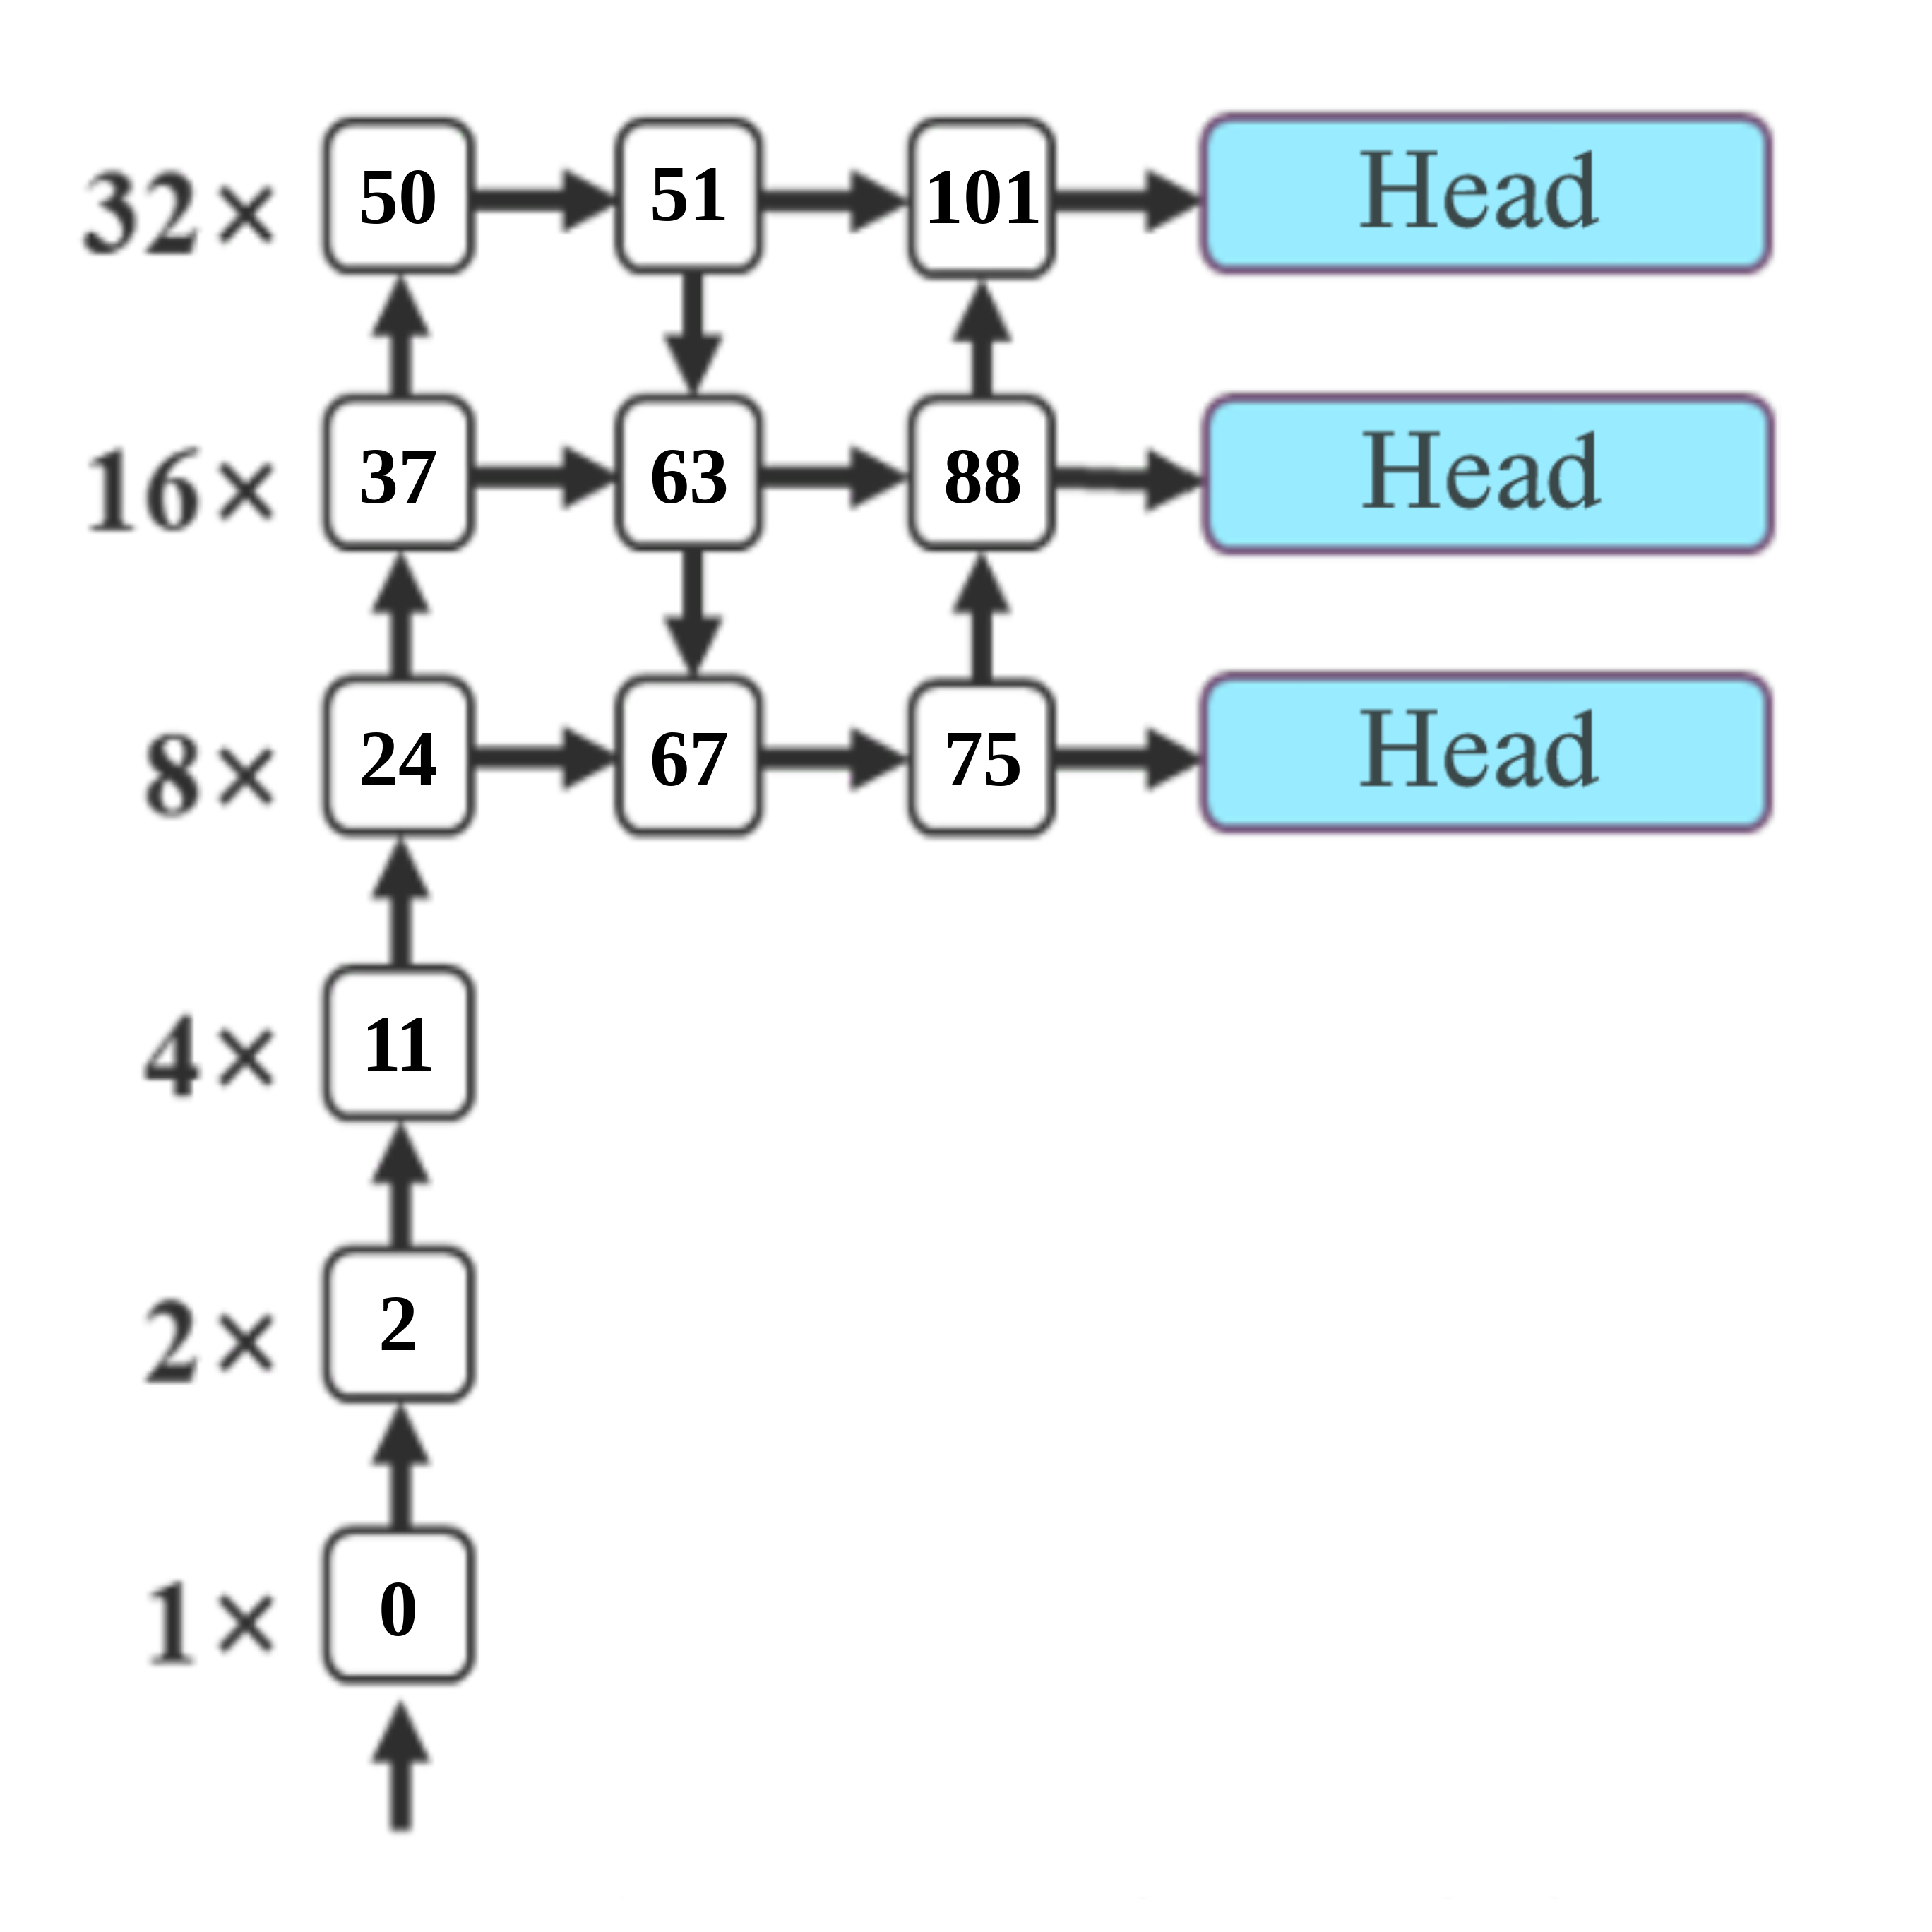
\includegraphics[width=1\linewidth]{figures/deeperconn-before.png}
      \caption{Before Rerouting}
      \label{fig:deeperconn-before}
    \end{subfigure}\hfill%\hspace{4em}
    \begin{subfigure}[][][t]{0.4\textwidth}
      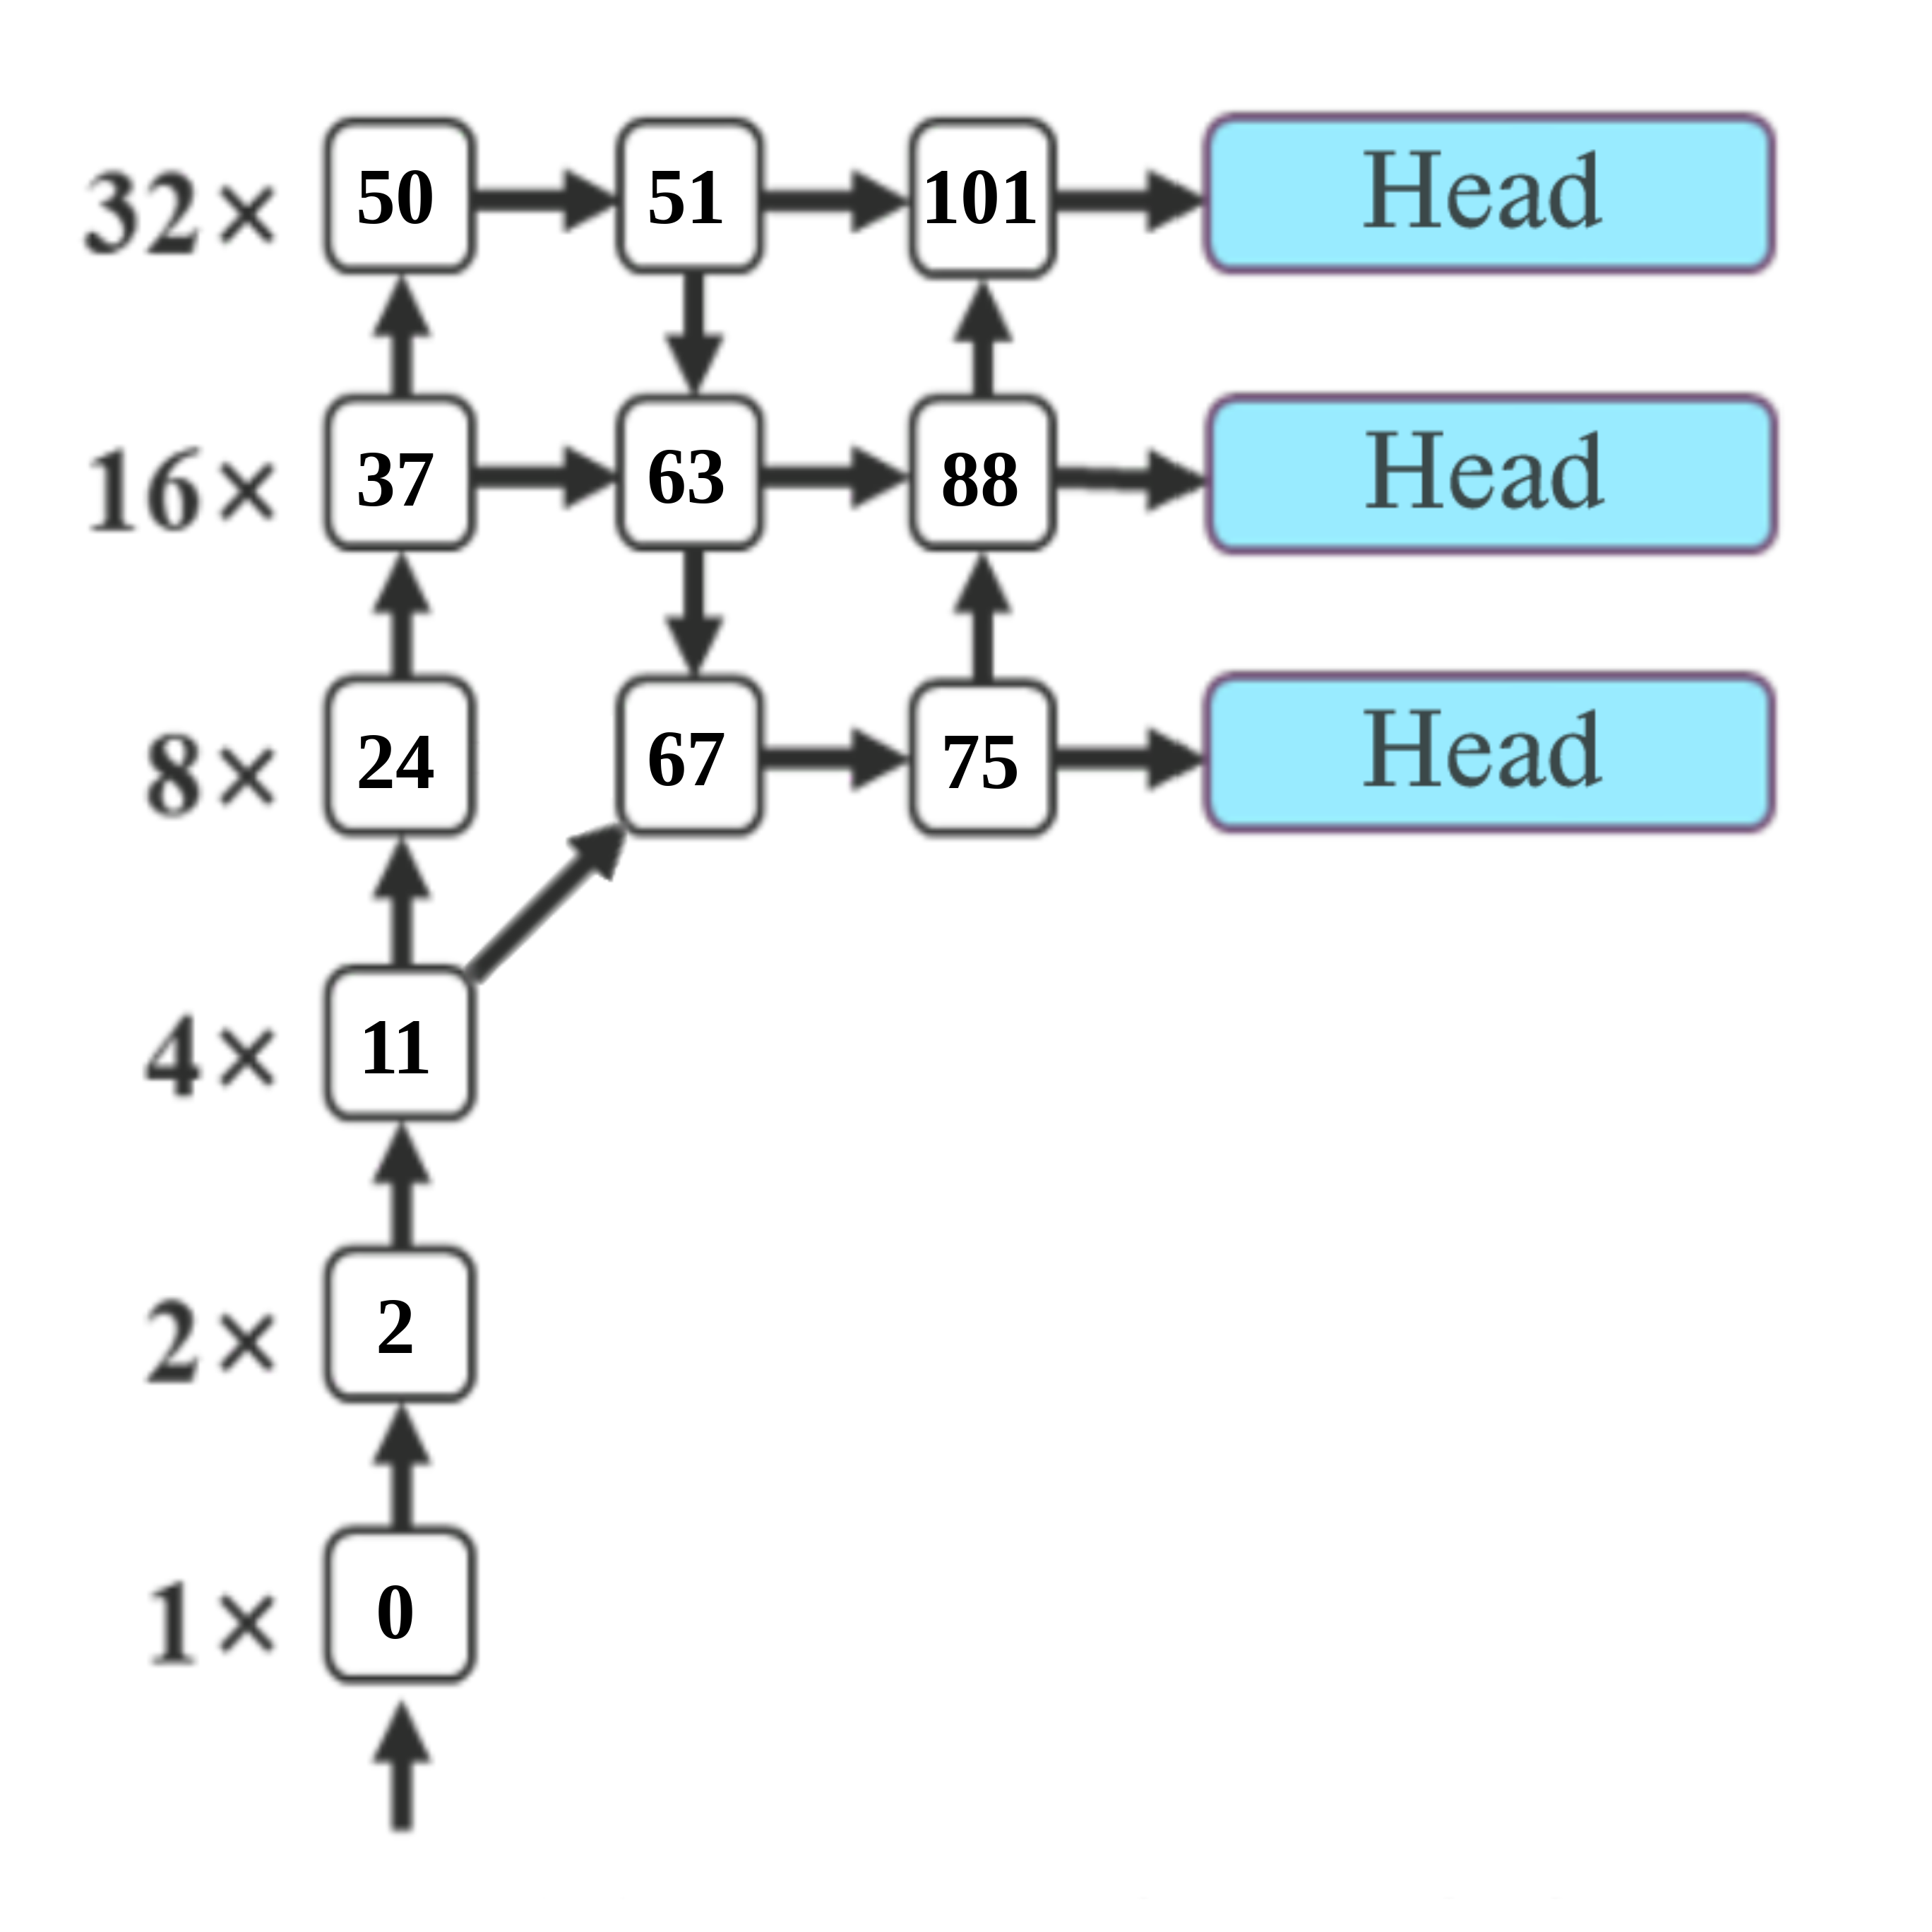
\includegraphics[width=1\linewidth]{figures/deeperconn-after.png}
      \caption{After Rerouting}
      \label{fig:deeperconn-after}
    \end{subfigure}
    \caption*{Adapted from: \textcite{yolov7} with permission (see Appendix \ref{appendix:license})}
    \caption{Modifying Connection to Earlier Feature Map Stage}
    \label{fig:deeperconn}
\end{figure}
%\begin{figure}[H]
%  \centering
%  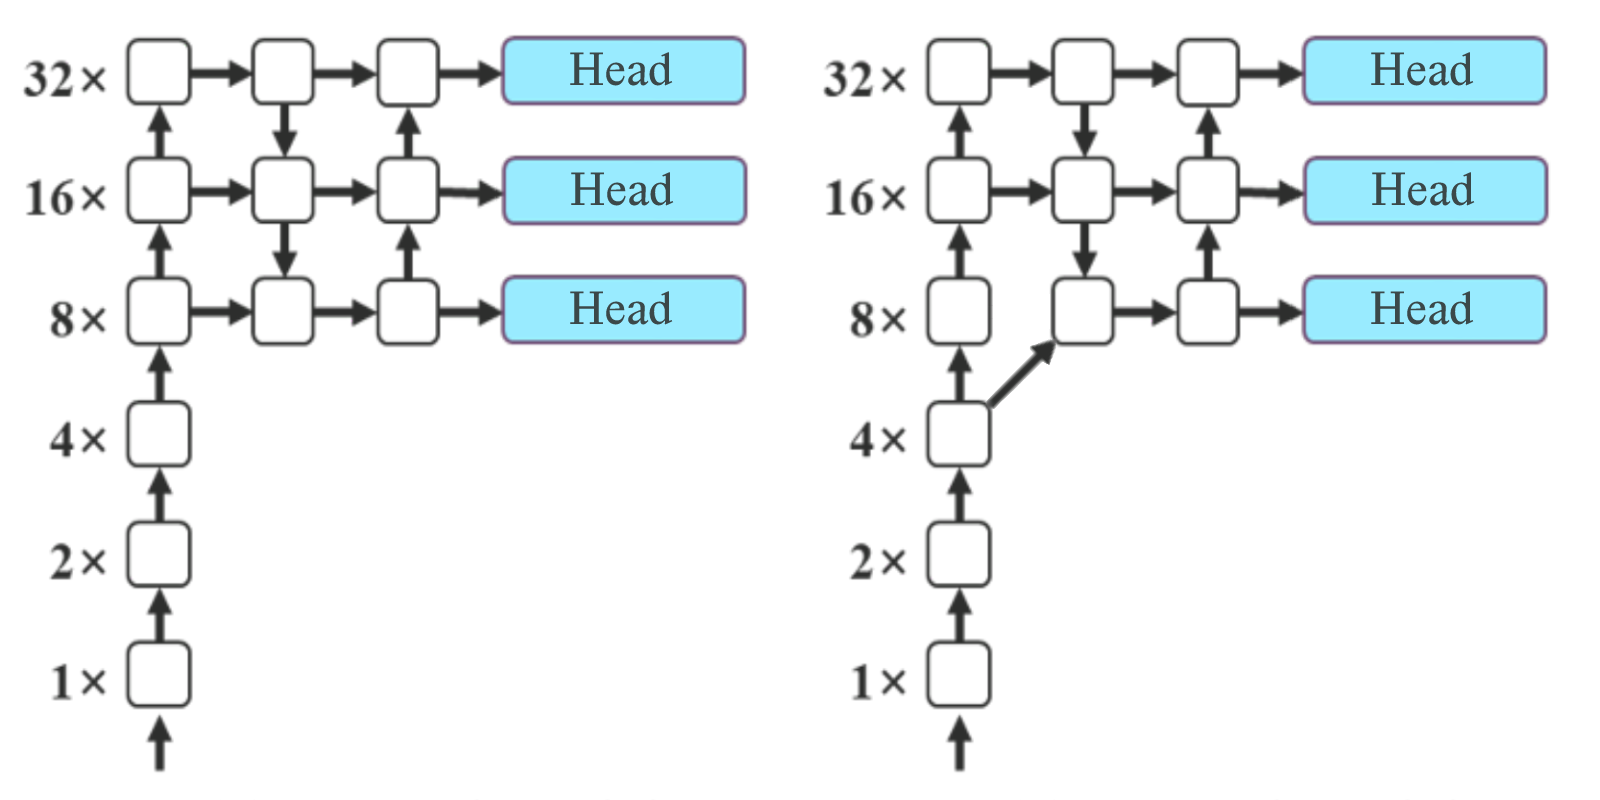
\includegraphics[width=0.7\textwidth]{figures/deeperconn.png}
%  \caption{Modifikasi Koneksi Neck. Kiri : Sebelum. Kanan : Sesudah.}
%  \label{fig:deeperconn}
%\end{figure}

As presented in Table \ref{tbl:neck_backbone_perf}, rerouting the source of 
feature map to an earlier stage produce an improvement of 2.98\% compared to \verb*|YOLOv7-MAR|.

\begin{table}
  \centering
  \captionof{table}{Performance of The Rerouted Model}
  \label{tbl:neck_backbone_perf}
  \vspace{-1ex}
    \begin{tabular}{ l l c }
    \toprule[1.5pt]
    No & Modification                                      &mAP@50 \\
    \midrule
    0  & \texttt{YOLOv7-MAR}                           & 11.2\%\\
    1  & \texttt{\textbf{YOLOv7-MAR + rerouting}} & \textbf{14.09\%}\\
    \midrule
       & Improvement                                & \textbf{\textcolor{green}{+2.98\%}}\\
    \bottomrule[1.5pt]
  \end{tabular}
\end{table}

%Perbandingan performa modifikasi ini dengan \verb*|YOLOv7-base| dapat dilihat pada tabel \ref{tbl:neck_backbone_perf}.
%Terlihat bahwa modifikasi ini berhasil meningkatkan skor mAP@50
%dari \verb*|YOLOv7-base| sebesar 2,98\%. Untuk mempermudah perbandingan dengan modifikasi lain, model hasil modifikasi
%ini akan disebut \verb*|YOLOv7-moveconnection|
\vspace{2ex}

\section{Additional YOLO Detection Head}
%Untuk modifikasi ini, pada skala 4 backbone, dipasangkan suatu layer head tambahan.
%Ilustrasi penambahan layer ini dapat dilihat pada gambar \ref{fig:addinghead}.
To add additional head layer, we utilized the feature map at the P2 scale of the network.
We introduced an upsampling block after layer 75 and fused it with layer 11 at layer 79 by concatenation.
To maintain the continuity of the network, we introduced a downsampling block that concludes at layer 87.
The subsequent layers in the network retained their original structure, but with layer numbering shifted by 25
as seen on Figure \ref{fig:addinghead}.
\begin{figure}
  \centering
  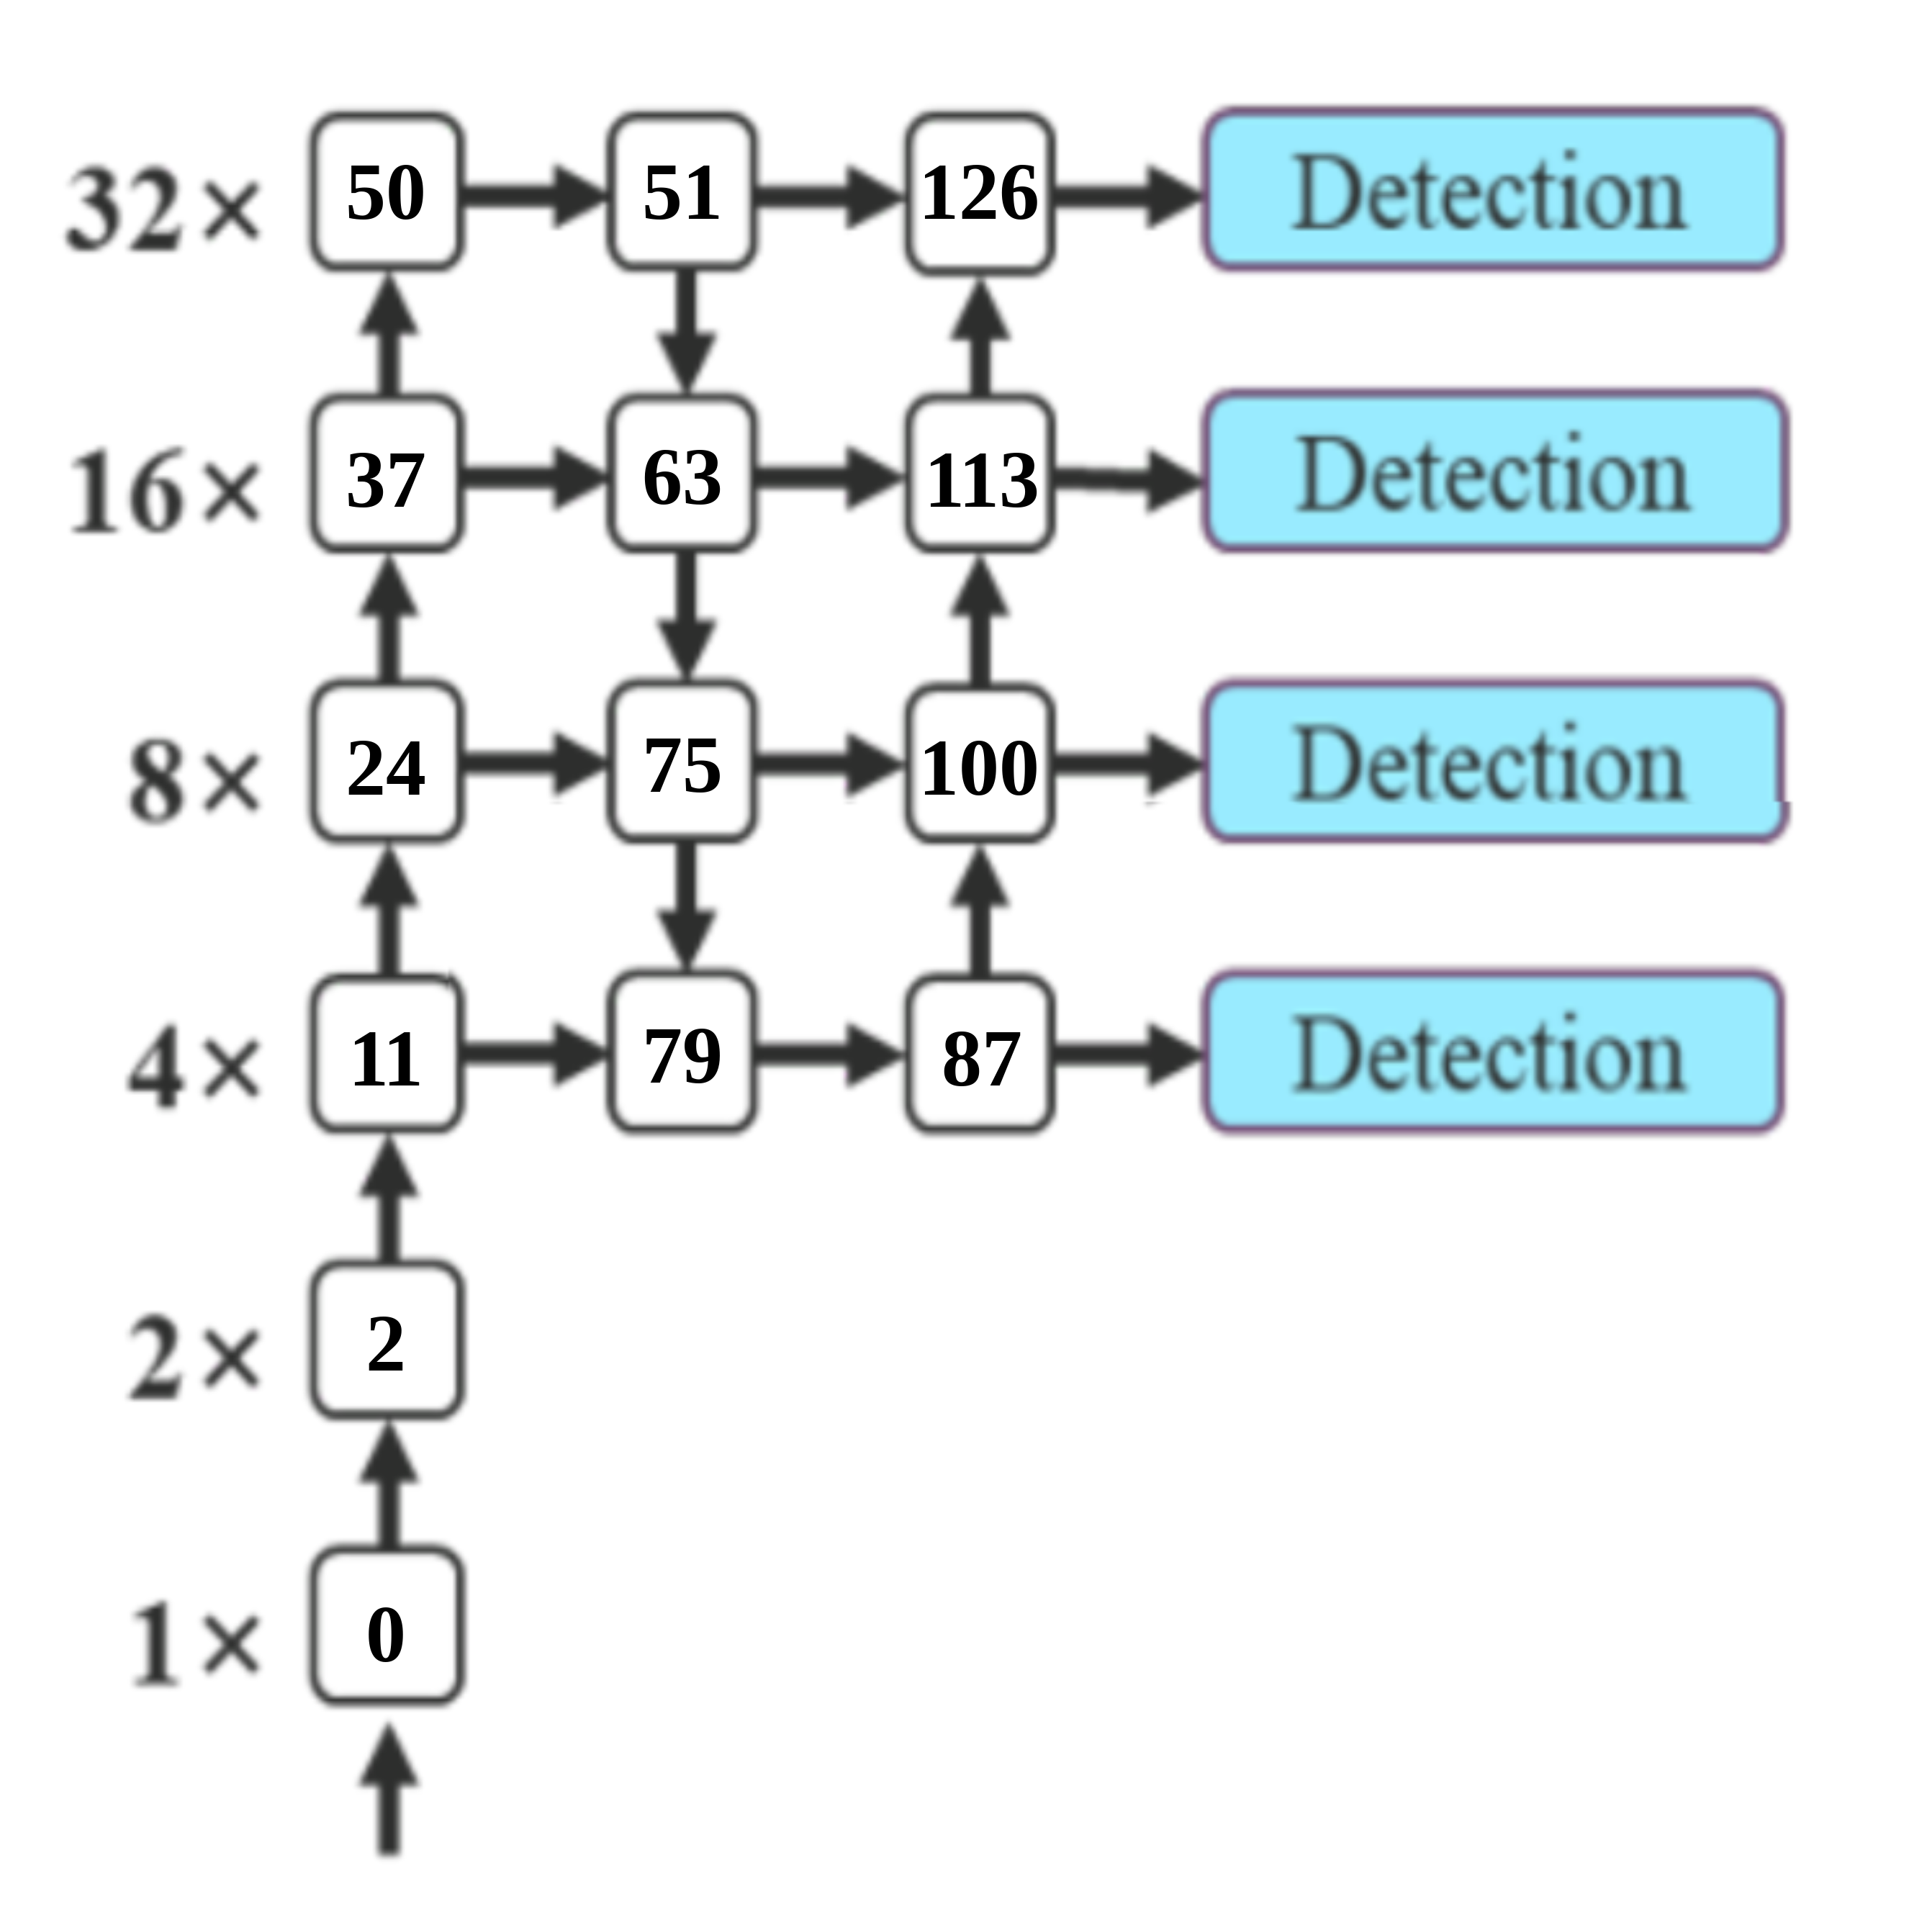
\includegraphics[width=0.35\textwidth]{figures/addheadn.png}
  \caption{Model Architecture After Increasing The Head}
  \label{fig:addinghead}
\end{figure}

\begin{table}
  \centering
  \captionof{table}{Additional Head Performance}
  \label{tbl:addhead}
  \vspace{-1ex}
    \begin{tabular}{ l l c }
    \toprule[1.5pt]
    No & Modifikasi                                 &mAP@50 \\
    \midrule
    0  & \texttt{YOLOv7-MAR}                        & \textbf{11.2\%}\\
    1  & \texttt{YOLOv7-MAR + more head}            & 5.19\%\\
    \midrule
       & Improvement                                & \textbf{\textcolor{red}{-6\%}}\\
    \bottomrule[1.5pt]
  \end{tabular}
\end{table}

As depicted in Table \ref{tbl:addhead}, additional head layer hurt the performance of the model.
This is counterintuitive. We had seen P2 feature map capable of increasing the mAP in previous section.
If we look at the loss at validation set, we can see that \verb|YOLO-MAR + head| is 
minimizing the localization loss more than \verb|YOLO-MAR + rerouting|.
There are several reasons we thought of why this happened:
\begin{enumerate}
  \item The network was simply producing loose bounding boxes prediction which looks better in loss function
  but fail when threshold criteria like in $mAP@50$ is introduced.

  \item This is an effect of bad choice of hyperparameters.
\end{enumerate}

%Seperti yang dapat dilihat pada tabel \ref{tbl:addhead}, penambahan modifikasi ini memberi performa 
%yang lebih buruk dibandingkan \verb*|YOLOv7-base|. 
%Padahal, modifikasi penambahan layer head dan \verb*|YOLOv7-moveconnection| dua-duanya menggunakan fitur pada skala 4.
%Alasan untuk hal ini akan diinvestiagsi dengan melihat output dari tiap skala pada model penambahan head dan \verb*|YOLOv7-moveconnection|.

\section{Decoupled Anchor-free Head}
%Penggantian \emph{head} menjadi \emph{decoupled anchor-free head} membuat model tidak mampu mendeteksi apapun pada dataset uji (mAP=0\%).
We experimented with replacing the coupled YOLO head to of a decoupled anchor-free head.
Upon replacing the head, we also replaced the label assigner from SimOTA to TAL.
The performance of this modification is shown in Table \ref{tbl:anchorfree_perf}.

The model was initially unable to converge due to numerical instability caused by having the objects becoming too small upon downscaling.
After stabilizing the loss function to handle these cases as shown in Appendix \ref{appendix:numerical-stabilization}, 
this modification was able to improve the mAP score by 21.78\%.

\begin{table}
  \centering
  \captionof{table}{Anchor-free Head Performance}
  \label{tbl:anchorfree_perf}
  \vspace{-1ex}
  \begin{tabular}{ l l c }
  \toprule[1.5pt]
  No & Model                                 &mAP@50 \\
  \midrule
  0  & \texttt{YOLOv7-MAR (anchor head)}        & \textbf{11.2\%}\\
  1  & \texttt{YOLOv7-MAR + anchor-free head}       & 0\% Bug Fix Data Coming Up\\
  \bottomrule[1.5pt]
\end{tabular}
\end{table}


\section{Partitioning Image}
{
\begin{figure}[p]
  \centering
  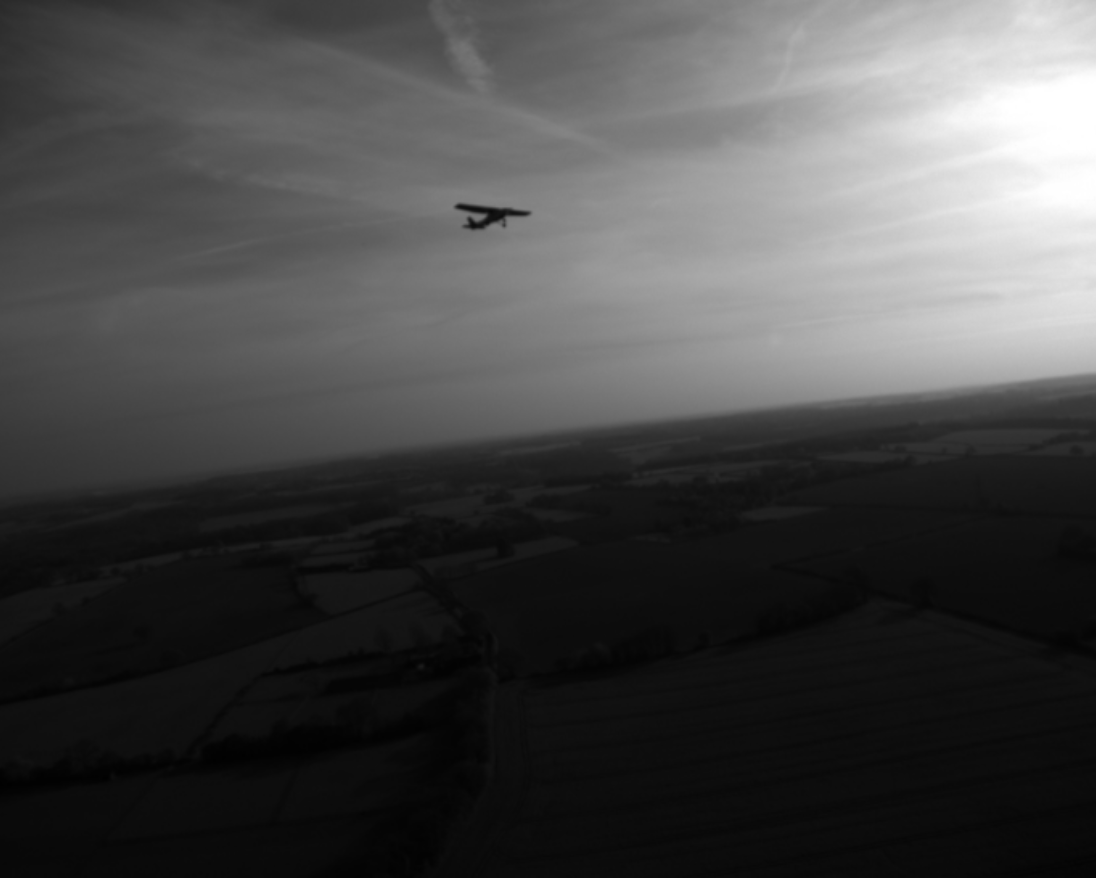
\includegraphics[height=0.33\textheight]{figures/crop_strat_source.png}
  \caption{Example Image Source for Cropping}
  \label{fig:crop-source}
\end{figure}
\begin{figure}[p]
  \centering
  \begin{subfigure}[][][t]{0.3\textwidth}
      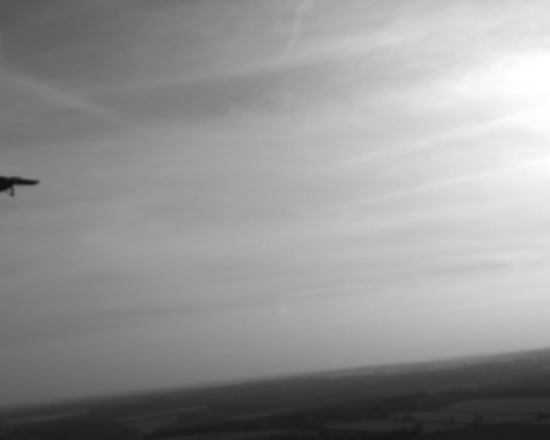
\includegraphics[width=1\linewidth]{figures/crop_strat_illegal1.png}
  \end{subfigure}
  \begin{subfigure}[][][t]{0.3\textwidth}
      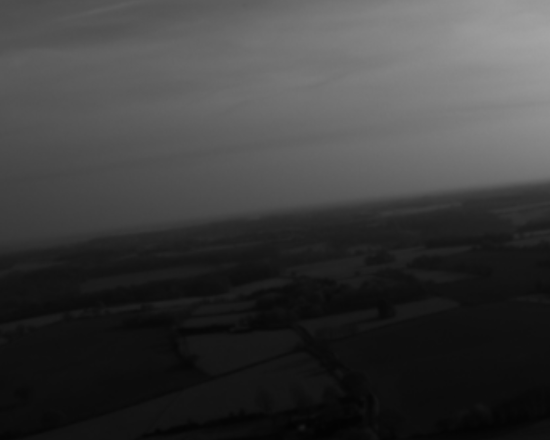
\includegraphics[width=1\linewidth]{figures/crop_strat_illegal2.png}
  \end{subfigure}
  \begin{subfigure}[][][t]{0.3\textwidth}
      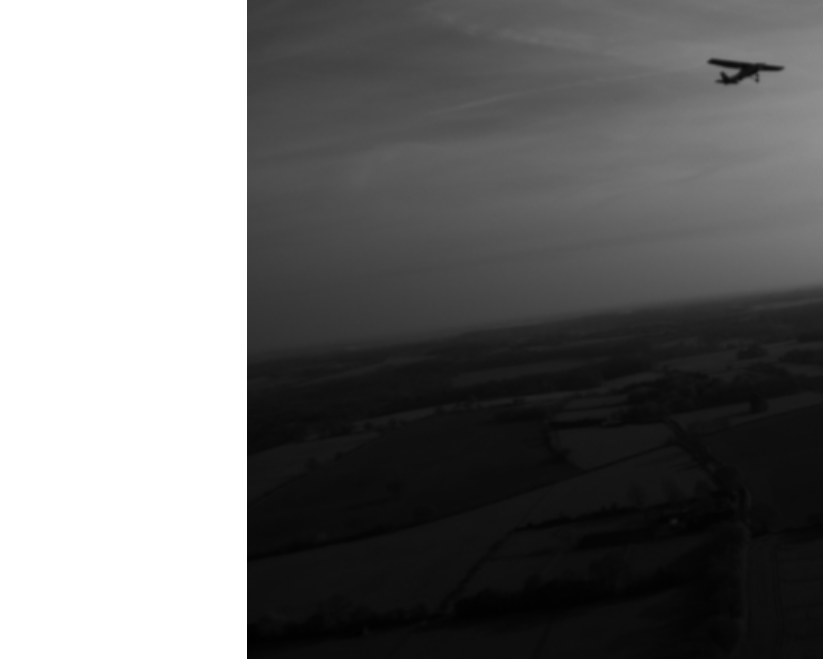
\includegraphics[width=1\linewidth]{figures/crop_strat_illegal3.png}
  \end{subfigure}
  \caption{Cropping without Strategy (Random Center)}
  \label{fig:crop-illegal}
\end{figure}
\begin{figure}[p]
  \centering
  \begin{subfigure}[][][t]{0.3\textwidth}
      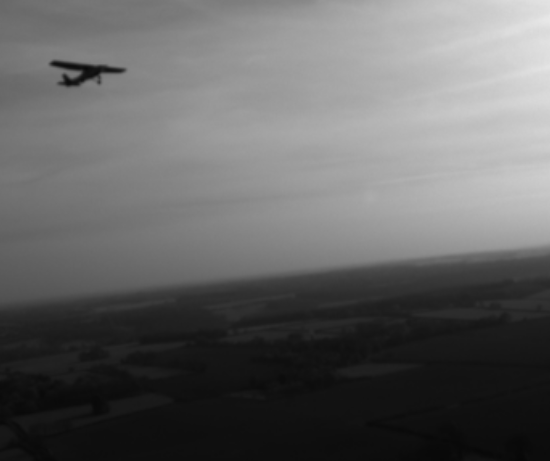
\includegraphics[width=1\linewidth]{figures/crop_strat_legal1.png}
  \end{subfigure}
  \begin{subfigure}[][][t]{0.3\textwidth}
      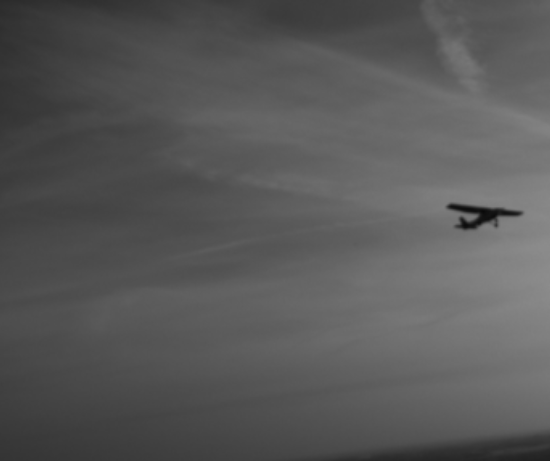
\includegraphics[width=1\linewidth]{figures/crop_strat_legal2.png}
  \end{subfigure}
  \begin{subfigure}[][][t]{0.3\textwidth}
      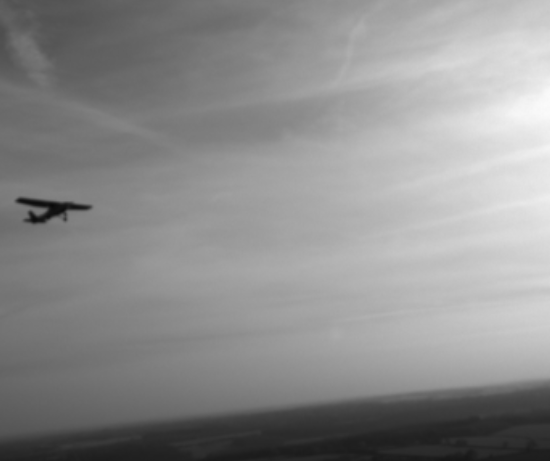
\includegraphics[width=1\linewidth]{figures/crop_strat_legal3.png}
  \end{subfigure}
  \caption{Cropping with Strategy}
  %\caption*{Cropping Strategy Guarantees the Existence of The Object}
  \label{fig:crop-legal}
\end{figure}
}
We trained the models using partitioned image of the original dataset.
In inference, we expect to partition an image into 4 equal sized images, which will
then be fed to the neural network. This way, the network will produce 4 independent
output that we can combine to form the final inference.

To generate partitioned data for training, we cropped image with size of $(W/2,H/2)$
based on the location of the objects bounding boxes. Therefore, it can be guaranteed that each image has at least
an object except for negative class images.
The procedure for this is described in the following:
\begin{itemize}[topsep=0pt]
  \item Open all images and their labels which consist of list of objects in it.
  \item For each object in an image, define a crop area with the following way:
  \begin{itemize}
    \item First, define the width and height of crop as a vector $\overrightarrow{crop_{wh}}$
    \item Then, we wanted to find a lower bound and upper bound for the x and y value that the crop center can be placed such that
    it would not cut object bounding box and not out of the boundary of the image itself. For example, for cropping the 
    image in Figure \ref{fig:crop-source}, we wanted to ensure the result would not be like in Figure \ref{fig:crop-illegal}.
    So, for the lower bound, we have:
      \begin{equation}
        \overrightarrow{crop_{lb}} = \max\left (\frac{\overrightarrow{c_{wh}}}{2} - \frac{\overrightarrow{crop_{wh}}}{2}, \frac{\overrightarrow{crop_{wh}}}{2} - \overrightarrow{c_{xy}}\right )
        \label{eq:partition-lb}
      \end{equation}
      \begin{align*}
        \text{Where}~c_{wh} &= \text{the width and height of the object's bounding box}\\
        c_{xy} &= \text{the center of the object's bounding box}\\
        \max(\vec{a},\vec{b}) &= \begin{pmatrix}\max(a.x,b.x) \\ \max(a.y,b.y)\end{pmatrix}  
      \end{align*}
    And for the upper bound:
      \begin{equation}
        \overrightarrow{crop_{ub}} = \max\left (\frac{\overrightarrow{crop_{wh}}}{2} - \frac{\overrightarrow{c_{wh}}}{2}  , 1 - \frac{\overrightarrow{crop_{wh}}}{2} - \overrightarrow{c_{xy}}\right )
        \label{eq:partition-ub}
      \end{equation}
    \item Finally, Equation \ref{eq:partition-lb} and \ref{eq:partition-ub} can be used to compute a randomized but constrained center point of the crop area
    by combining them to the following equation:
    \begin{equation}
      \overrightarrow{crop_{xy}} = \text{diag}(R)(\overrightarrow{crop_{ub}} - \overrightarrow{crop_lb}) + \overrightarrow{crop_{lb}} + \overrightarrow{c_{xy}}
    \end{equation}
    \begin{align*}
      \text{Where}~R &= \text{a random vector with value of its element is within $(0,1)$}\\
      \text{diag}(R) &= \text{a function that convert a vector $R$ to a diagonal matrix with elements of}\\ &\text{ R as its diagonal}\\
    \end{align*}
  \end{itemize}
  \item After the cropping area has been defined, the bounding boxes' values must also be converted to the cropped perspective.
  These conversions were done like the following:
  \begin{align}
    \overrightarrow{\hat{c}_{xy}} &= \overrightarrow{c_{xy}} - (\overrightarrow{crop_{xy}} - \frac{\overrightarrow{crop_{wh}}}{2})\\
    \overrightarrow{\hat{c}_{wh}} &= \frac{\overrightarrow{c_{wh}}}{\overrightarrow{crop_{wh}}} \label{eq:partition-wh-conversion}
  \end{align}
  Where the division operation in Equation \ref{eq:partition-wh-conversion} is an element-wise division, meaning the x component of the numerator is divided by the x component of the denominator, likewise for y component.
\end{itemize}
By following this procedure, it is ensured that the cropping for training image would be like in Figure \ref{fig:crop-legal} and not like Figure \ref{fig:crop-illegal}.
Without using this strategy, the resulting partitioned image for training would have a significant increase in negative class that could reduce the neural network recall ability.

The procedure so far only consider for the case when the objects are about $crop_{wh}$ away from each other.
If the objects are within $crop_{wh}$ from each other, we redefined the $c_{xy}$ and $c_{wh}$ to be the smallest box
that bounds every object in the image. Redefinition is done in the following way:
\begin{align}
  \text{Let}~B &= \text{set bounding boxes in an image} \nonumber \\
  c_{tl}.x &= \min \{c^*_{tl}.x : \forall\ c^* \in B\} \nonumber \\
  c_{tl}.y &= \min \{c^*_{tl}.y : \forall\ c^* \in B\}\nonumber \\
  c_{br}.x &= \max \{c^*_{br}.x : \forall\ c^* \in B\}\nonumber \\
  c_{br}.y &= \max \{c^*_{br}.y : \forall\ c^* \in B\}\nonumber \\
  c_{xy} &= \frac{c_{br}+c_{tl}}{2} \label{eq:partition-newcxy}\\
  c_{wh} &= c_{br}-c_{tl} \label{eq:partition-newcwh}
\end{align}

Since the image were partitioned to a  smaller size, we were finally able to use a smaller input size 
for the neural network. We experimented by using 640 and 960 input size on some previous modifications.
The performance is shown on Table \ref{tbl:partition-perf}.
\verb|YOLOv7-MAR + anchor-free| with input size 960 produced the greatest mAP@50 score
amongst other model when partitioned to 4.



\begin{table}[b]
  \centering
  \captionof{table}{Partitioning Image Performance}
  \label{tbl:partition-perf}
  \vspace{-1ex}
  \begin{tabular}{ l l c c c}
  \toprule[1.5pt]
  No & Model                                       &  Input Size  &Partition4 mAP@50               &mAP@50\\
  \midrule
  0  & \texttt{YOLOv7-AR}                          &     960      & 2.9\%                          &TBA\\
  1  & \texttt{YOLOv7-MAR}                         &     640      & 18.46\%                        &TBA\\
  3  & \texttt{YOLOv7-MAR}                         &     960      & 37.69\%                        &TBA\\
  4  & \texttt{YOLOv7-MAR + rerouting}             &     960      & 30.04\%                        &TBA\\
  5  & \texttt{YOLOv7-MAR + more head}             &     960      & 10.53\%                        &TBA\\
  6  & \texttt{YOLOv7-MAR + anchor-free}           &     640      & 37.57\%                        &TBA\\
  7  & \texttt{\textbf{YOLOv7-MAR + anchor-free}}  &     960      &\textbf{46.18\%}                &TBA\\
  %\midrule
  %   & Improvement                                 &              & \textbf{\textcolor{red}{-6\%}} &TBA\\
  \bottomrule[1.5pt]
\end{tabular}
\end{table}

\section{Latency}
In this section, the latency of the modifications is presented.
The data obtained using computer with specification presented in section \ref{section:instrument}.
Table \ref{tbl:inference-speed} shows that all the partition 4 models have $> 40$ FPS inference speed.
This means that they are able to perform at $>10$ FPS even without batching to detect a full image, making them all valid candidate for the best model.


\begin{table}
  \centering
  \captionof{table}{Inference Speed of Modified Models}
  \label{tbl:inference-speed}
  \vspace{-1ex}
  \begin{adjustbox}{width=\textwidth}
  \begin{tabular}{ l l c c c}
  \toprule[1.5pt]
  No & Model                                       &   Input Size         &\multicolumn{2}{c}{Inference Speed}                   \\
     &                                             &                      &Not Reparameterized  &  Reparameterized   \\
  \midrule
  0  & \texttt{YOLOv7-MAR, plain, M, AR, EIoU}     &      1600            & 29.6 FPS            & TBA   \\
  1  & \texttt{YOLOv7-MAR + rerouting}             &      1600            & 23.28 FPS           & TBA   \\
  2  & \texttt{YOLOv7-MAR + more head}                 &      1600            & 15.91 FPS           & TBA   \\
  3  & \texttt{YOLOv7-MAR + anchor-free}               &      1600            & TBA                 & TBA   \\
  \midrule
  4  & \texttt{YOLOv7-MAR}                         &  Partition 4, 960    & TBA                 & TBA   \\
  5  & \texttt{YOLOv7-MAR + rerouting}             &  Partition 4, 960    & TBA                 & TBA   \\
  6  & \texttt{YOLOv7-MAR + more head}             &  Partition 4, 960    & TBA                 & TBA   \\
  7  & \texttt{YOLOv7-M + anchor-free}           &  Partition 4, 960    & TBA                 & TBA   \\
  \midrule
  8  & \texttt{YOLOv7-MAR}                         &  Partition 4, 640    & TBA                 & TBA   \\
  9  & \texttt{YOLOv7-MAR + rerouting}             &  Partition 4, 640    & TBA                 & TBA   \\
  10 & \texttt{YOLOv7-MAR + more head}             &  Partition 4, 640    & TBA                 & TBA   \\
  11 & \texttt{YOLOv7-M + anchor-free}           &  Partition 4, 640    & TBA                 & TBA   \\
  %\midrule
  %   & Improvement                                 &              & \textbf{\textcolor{red}{-6\%}} &TBA\\
  \bottomrule[1.5pt]
\end{tabular}
  \end{adjustbox}

\end{table}

